\chapter{Sprint 2: Uni-match}



\section*{Introduction}

\addcontentsline{toc}{section}{Introduction}

In this chapter, we'll be exploring the second Sprint, which focuses on the design and implementation of uni-world's social features.

\section{Sprint Backlog}
To start, we outline the work to be done in this sprint. The schedule for this iteration
involves the user stories described in the following Table 3.1:

\begin{longtable}{|l|p{6cm}|p{8cm}|}
\hline
Sprint & User story & Task\\
\hline
\endfirsthead

\multicolumn{3}{c}{{\bfseries}} \\
\hline
Sprint & User story & Task\\
\hline
\endhead

\hline \multicolumn{3}{|r|}{{Continued on next page}} \\ \hline
\endfoot

\hline
\endlastfoot
3 & As a student, I want to show my interest by swiping right on someone
so that I can contact them if they like me back & \begin{itemize}
    \item Create the like and match models
    \item Create the algorithm responsible for showing the users
    \item Create the matching system
    \item Create the matching feed UI
    \item Integration and testing
\end{itemize} \\ \hline

4 & As a student, I want to ignore someone I don’t find interesting & \begin{itemize}
    \item Create ignoring feature
    \item enhancing the algorithm
    \item Integration and testing
\end{itemize} \\ \hline

7 & As a student, I want to send and receive messages from my matches & \begin{itemize}
    \item Create a web socket to handle real-time communication
    \item Create the message and conversation models
    \item Create messaging feature
    \item Create messaging UI
    \item Integration and testing
\end{itemize} \\ \hline

8 & As a student, I want to see who likes me so I can decide whether or
not to like them back & \begin{itemize}
    \item Create the likes UI
    \item Integration and testing
\end{itemize} \\ \hline

9 & As a student, I want to filter my feed according to many criteria & \begin{itemize}
    \item Create user preferences schema
    \item Create filtering feature 
    \item Create filtering UI 
    \item Integration and testing
\end{itemize} \\ \hline

10 & As a student, I want to choose the gender I want to interact with & \begin{itemize}
    \item Update filtering UI 
    \item Integration and testing
\end{itemize} \\ \hline
\caption{Sprint 2 backlog}
\label{Tab: Sprint 2 backlog}
\end{longtable}


\section{ Analysis and conception}
In this section, we illustrate the sprint analysis in a more visual representation using use case diagrams and sequence diagrams of the most highlighted features:
"profiles browsing" and "Likes management".

\subsection{Use case diagrams}
\textbf{Refined use case diagram for profiles browsing: }
\begin{figure}[H] 
            \centering
            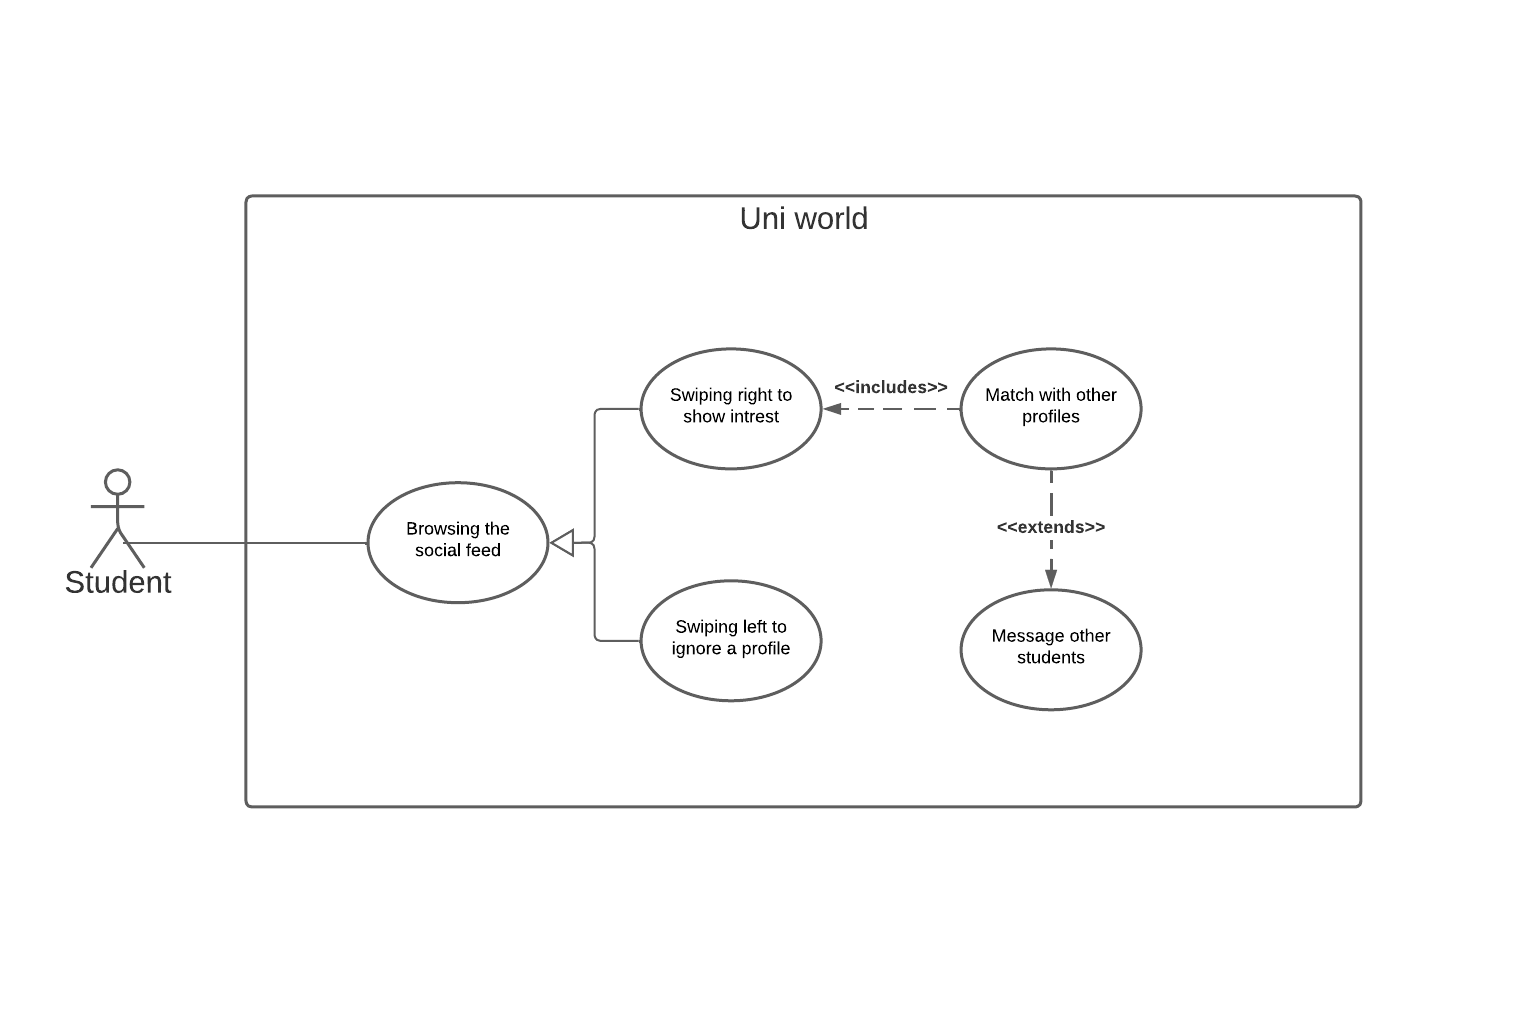
\includegraphics[scale=0.6]{diagrams/refined use case social swipe.png}
            \caption{Refined use case diagram for profiles browsing} 
            \label{fig: Refined use case diagram for profiles browsing}
\end{figure}

The diagram of the "Likes management" use case is shown in figure 3.2 :

\begin{figure}[H] 
            \centering
            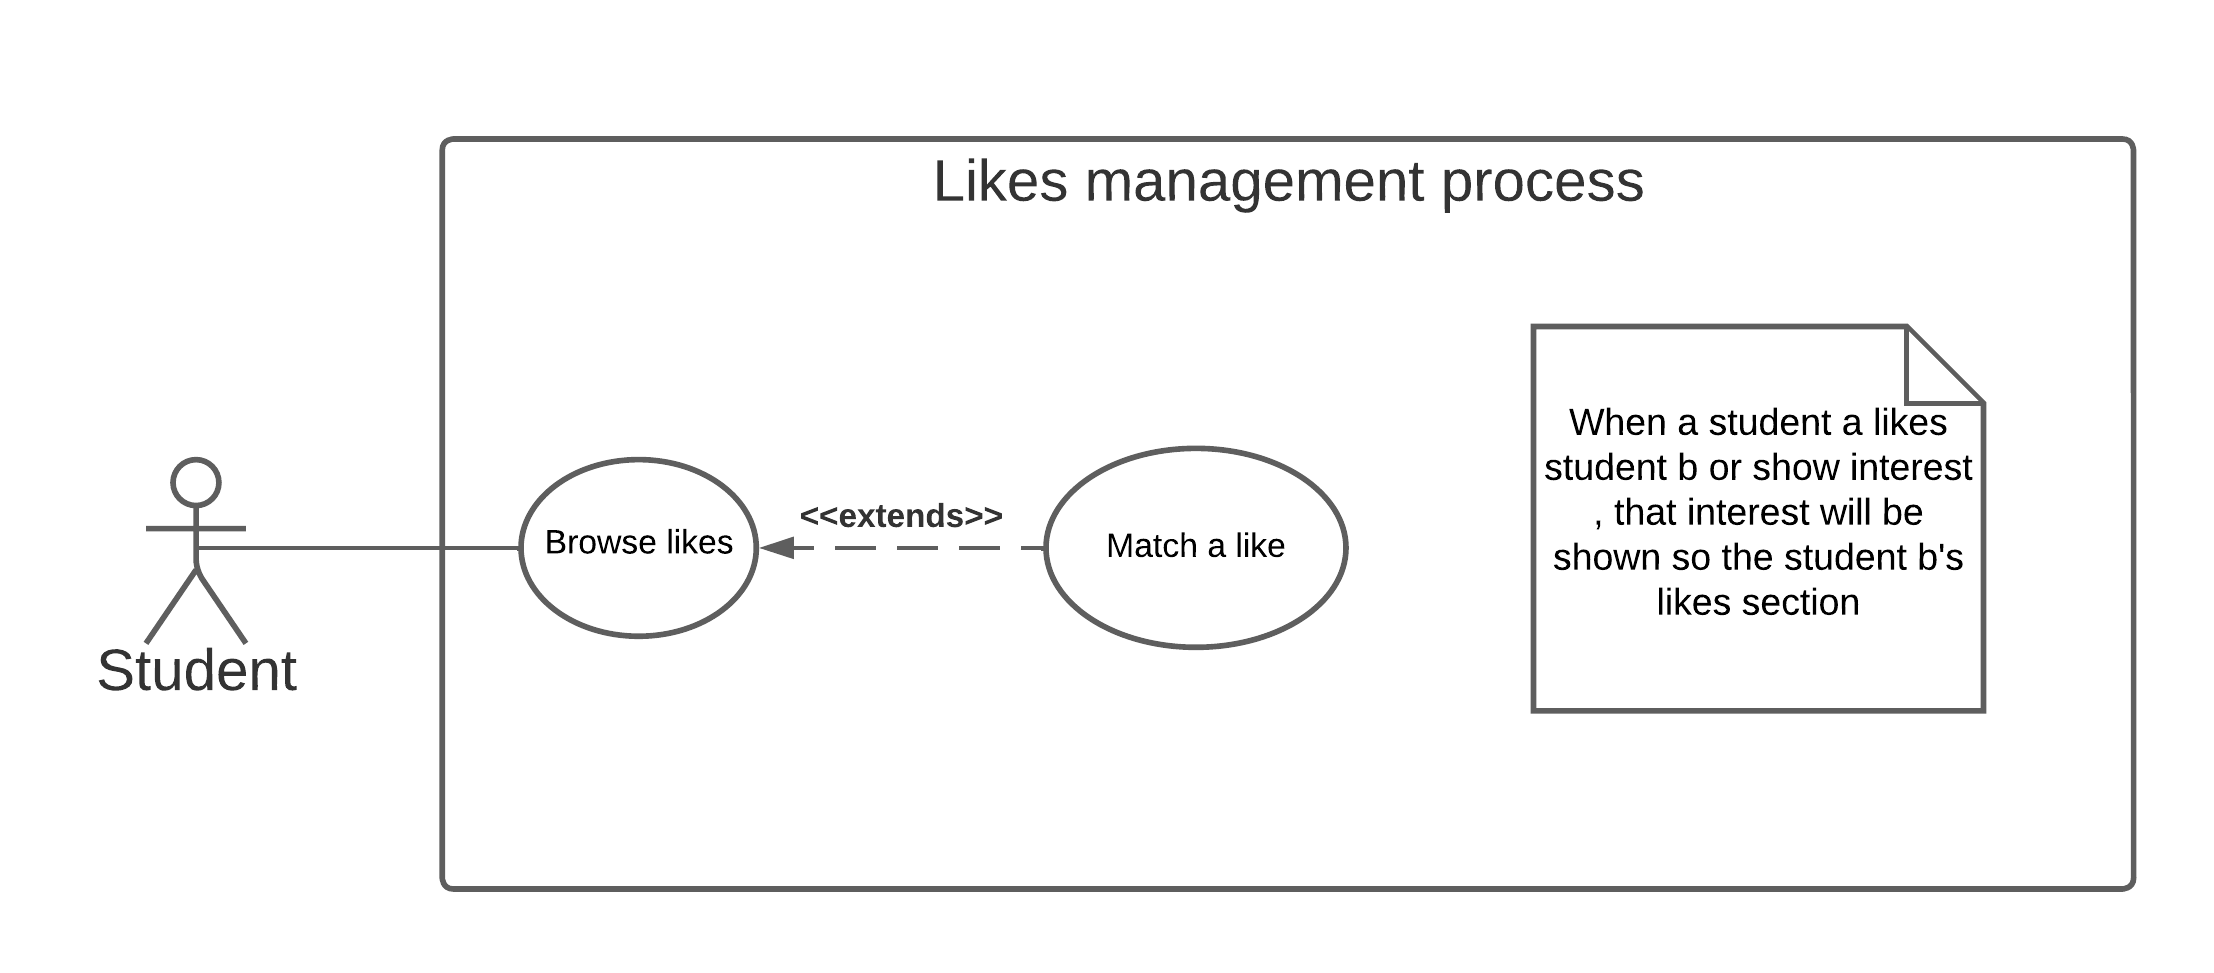
\includegraphics[scale=0.8]{diagrams/likes management use case.png}
            \caption{Likes management use case diagram} 
            \label{fig: Likes management use case diagram}
\end{figure}

\subsection{Use case textual descriptions}
Textual descriptions of the "profiles browsing" use case are illustrated in table 4.2 below:
\begin{longtable}{|c|p{10cm}|}
\hline
Use Case & Description \\\hline
Name & profiles browsing use case \\\hline
Preconditions & the student must be authenticated and have an active account \\\hline
Postconditions & After matching, the student can send a message of his/her choice to the other students who are in the system. This communication function mainly helps profiles that are matched to be able to communicate effectively. \\ \hline
Main Flow & 
\begin{enumerate}
    \item Student opens the feed screen.
    \item   Student passes through the profiles with the help of the system known as “Uni match”
    \item Such action enables them to see the profiles of other users and get two choices:
        \begin{itemize}
            \item   Swipe right: Expresses the student’s liking for a profile.
            \item   Swipe left: Fails to heed a profile.
        \end{itemize} 
        \item the action will be incorporated into the system. 
        \item The selected profiles are “matched”.
\end{enumerate}

\\\hline
Alternative Flows & 
    if there is a network error, an error message appears
\\\hline
\caption{Textual descriptions of the profiles browsing use case}
\label{Tab: Textual descriptions of the profiles browsing use case}
\end{longtable}

The use case textual description of "Likes management" is illustrated in the
following Table 3.3:

\begin{longtable}{|c|p{10cm}|}
\hline
Use Case & Description \\\hline
Name & Likes management use case \\\hline
Preconditions & user A and User B must both have an active account and must both be authenticated \\\hline
Postconditions & user A and User B can match if user A likes User B back
\\\hline
Main Flow &
Let's suppose we have two users A and B
\begin{enumerate}
    \item User A will swipe right (shows interest) to user B
    \item User B will receive a new like in his likes section 
    \item User B can
       \begin{itemize}
        \item Return the like to User A so they can match
        \item Ignore the like so it can eventually disappear once he swipes left on user A's profile in the feed
    \end{itemize} 
\end{enumerate}
\\\hline
Alternative Flows & \begin{itemize}
    \item if User B swipes left (ignores) User A profile, the like will be automatically deleted
    \item if there is a network error, an error message appears
\end{itemize}
\\\hline
Non-functional Requirements & \begin{itemize}
    \item The Like management will have a user-friendly UI
\end{itemize}
\\\hline
\caption{Textual descriptions of the Likes management use case}
\label{Tab: Textual descriptions of the Likes management use case}
\end{longtable}

\subsection{Sequences diagram}
The Profiles browsing object sequence diagram can be observed in Figure 4.3 below:

\begin{figure}[H] 
            \centering
            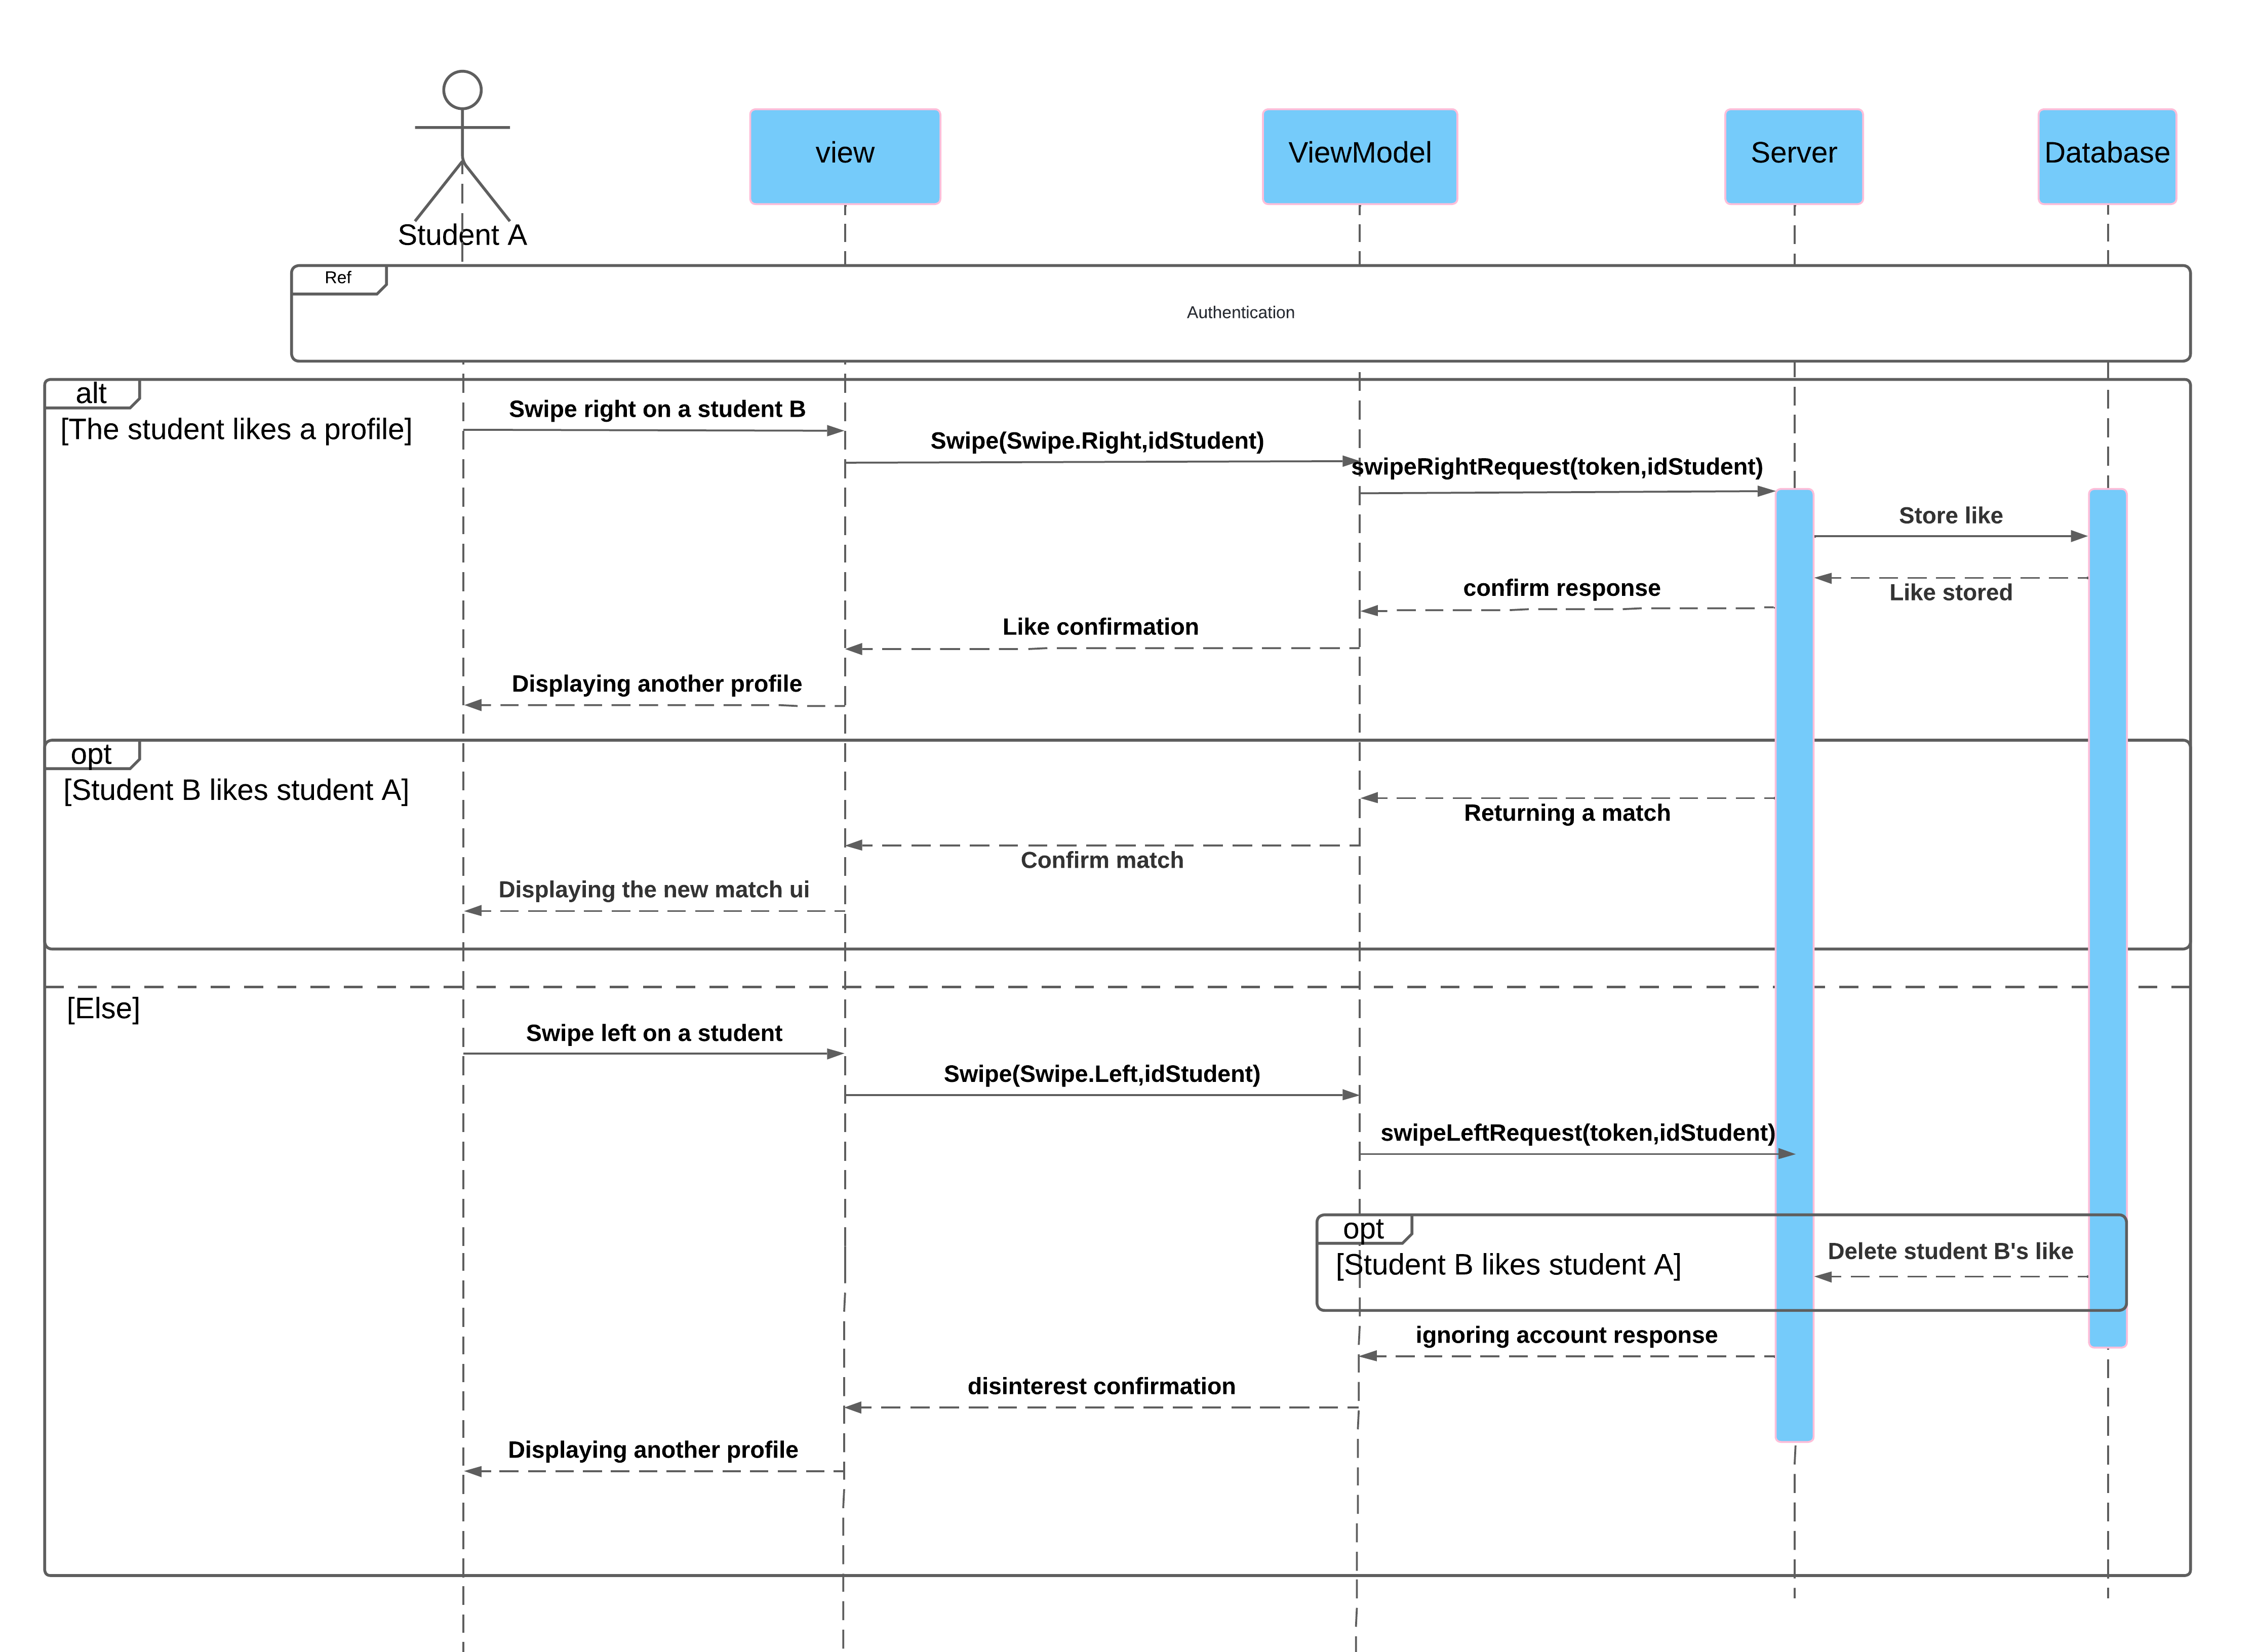
\includegraphics[scale=0.4]{diagrams/profile browsing seq diagram.png}
            \caption{Profiles browsing object sequence diagram} 
            \label{fig: Profiles browsing object sequence diagram}
\end{figure}

The Likes management system system sequence diagram can be observed in Figure 4.4 below:

\begin{figure}[H] 
            \centering
            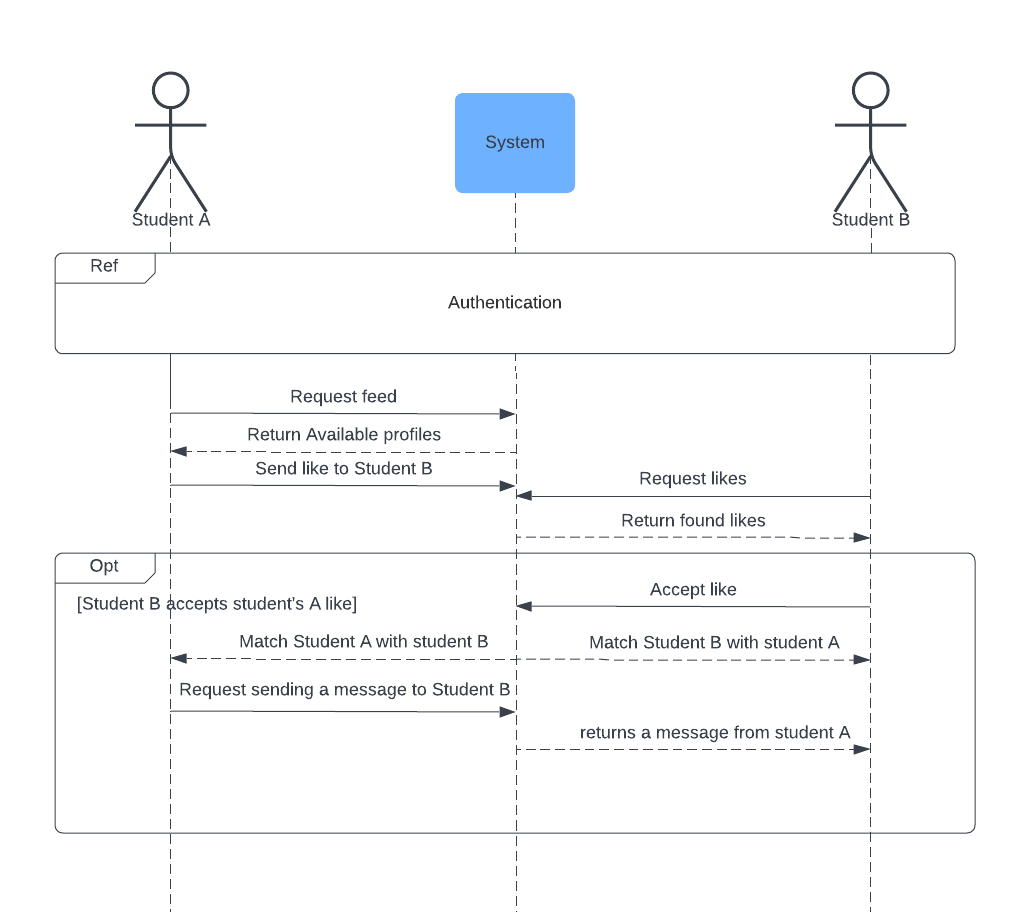
\includegraphics[scale=0.7]{diagrams/Sequence diagram like management.png}
            \caption{Likes management system sequence diagram} 
            \label{fig: Likes management system sequence diagram}
\end{figure}

\section{Realization}
In this section, we describe what has been implemented and how the various components and functionalities identified in this Sprint have been instantiated.

\subsection{Uni-match feed and profiles browsing}

With the User needs in mind, the flow for socializing as well as selecting users to connect with is quite friendly and simple to navigate. from a simple motion which is a swipe. similar to this, users can just swipe right to mean they would like to get connected with the other user or just swipe left to reject the other user. When two users have shown their interest towards each other the system tends to recommend the two users as being fit to be partners and thus they are allowed to-chat.\\

Below, we take a look at the matching feed where the user can swipe on different profiles. \\
\begin{figure}[H] 
            \centering
            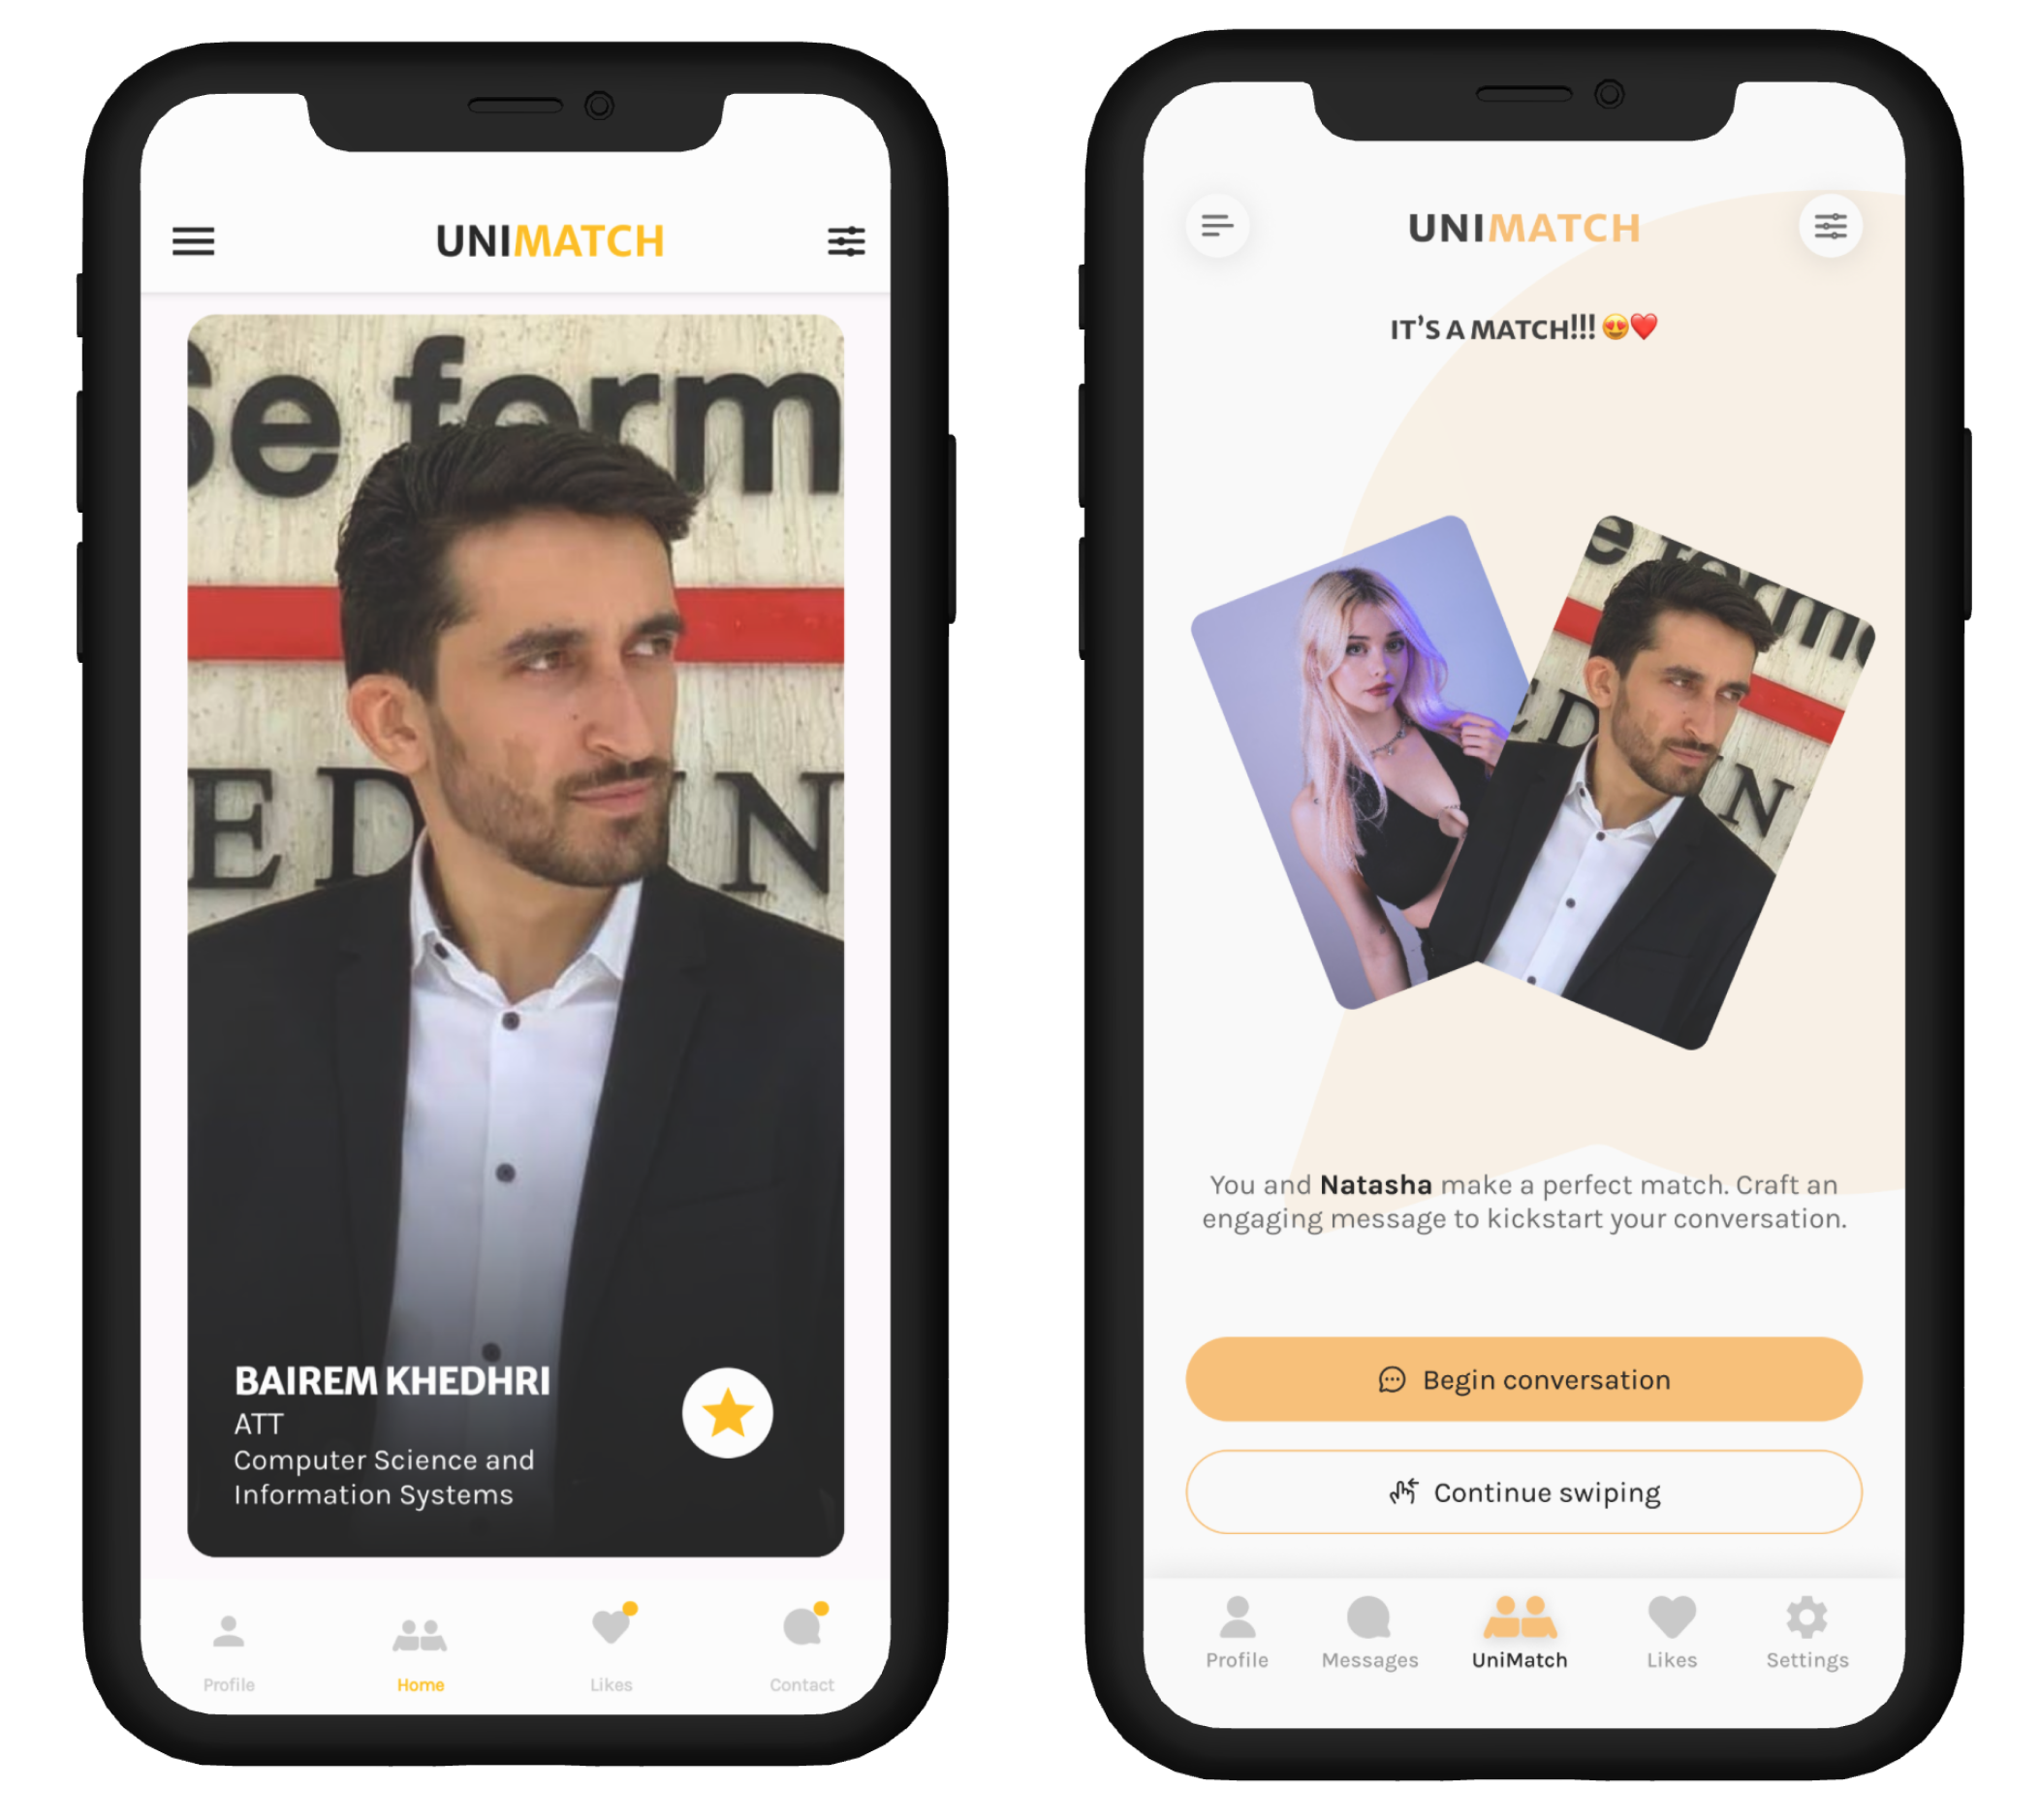
\includegraphics[scale=0.2]{feed ui.png}
            \caption{Some Feed UIs} 
            \label{fig: Feed UI}
\end{figure}

\subsection{Messaging features}
This is as we mentioned above, in the previous sub-section, each time two users match because of the interest they have in each other, they can then send each other a message in the messaging area.

Below this there is the Contacts interface where users can find the list of matches and chats, and to the right we'll find the Chat interface .
\begin{figure}[H] 
            \centering
            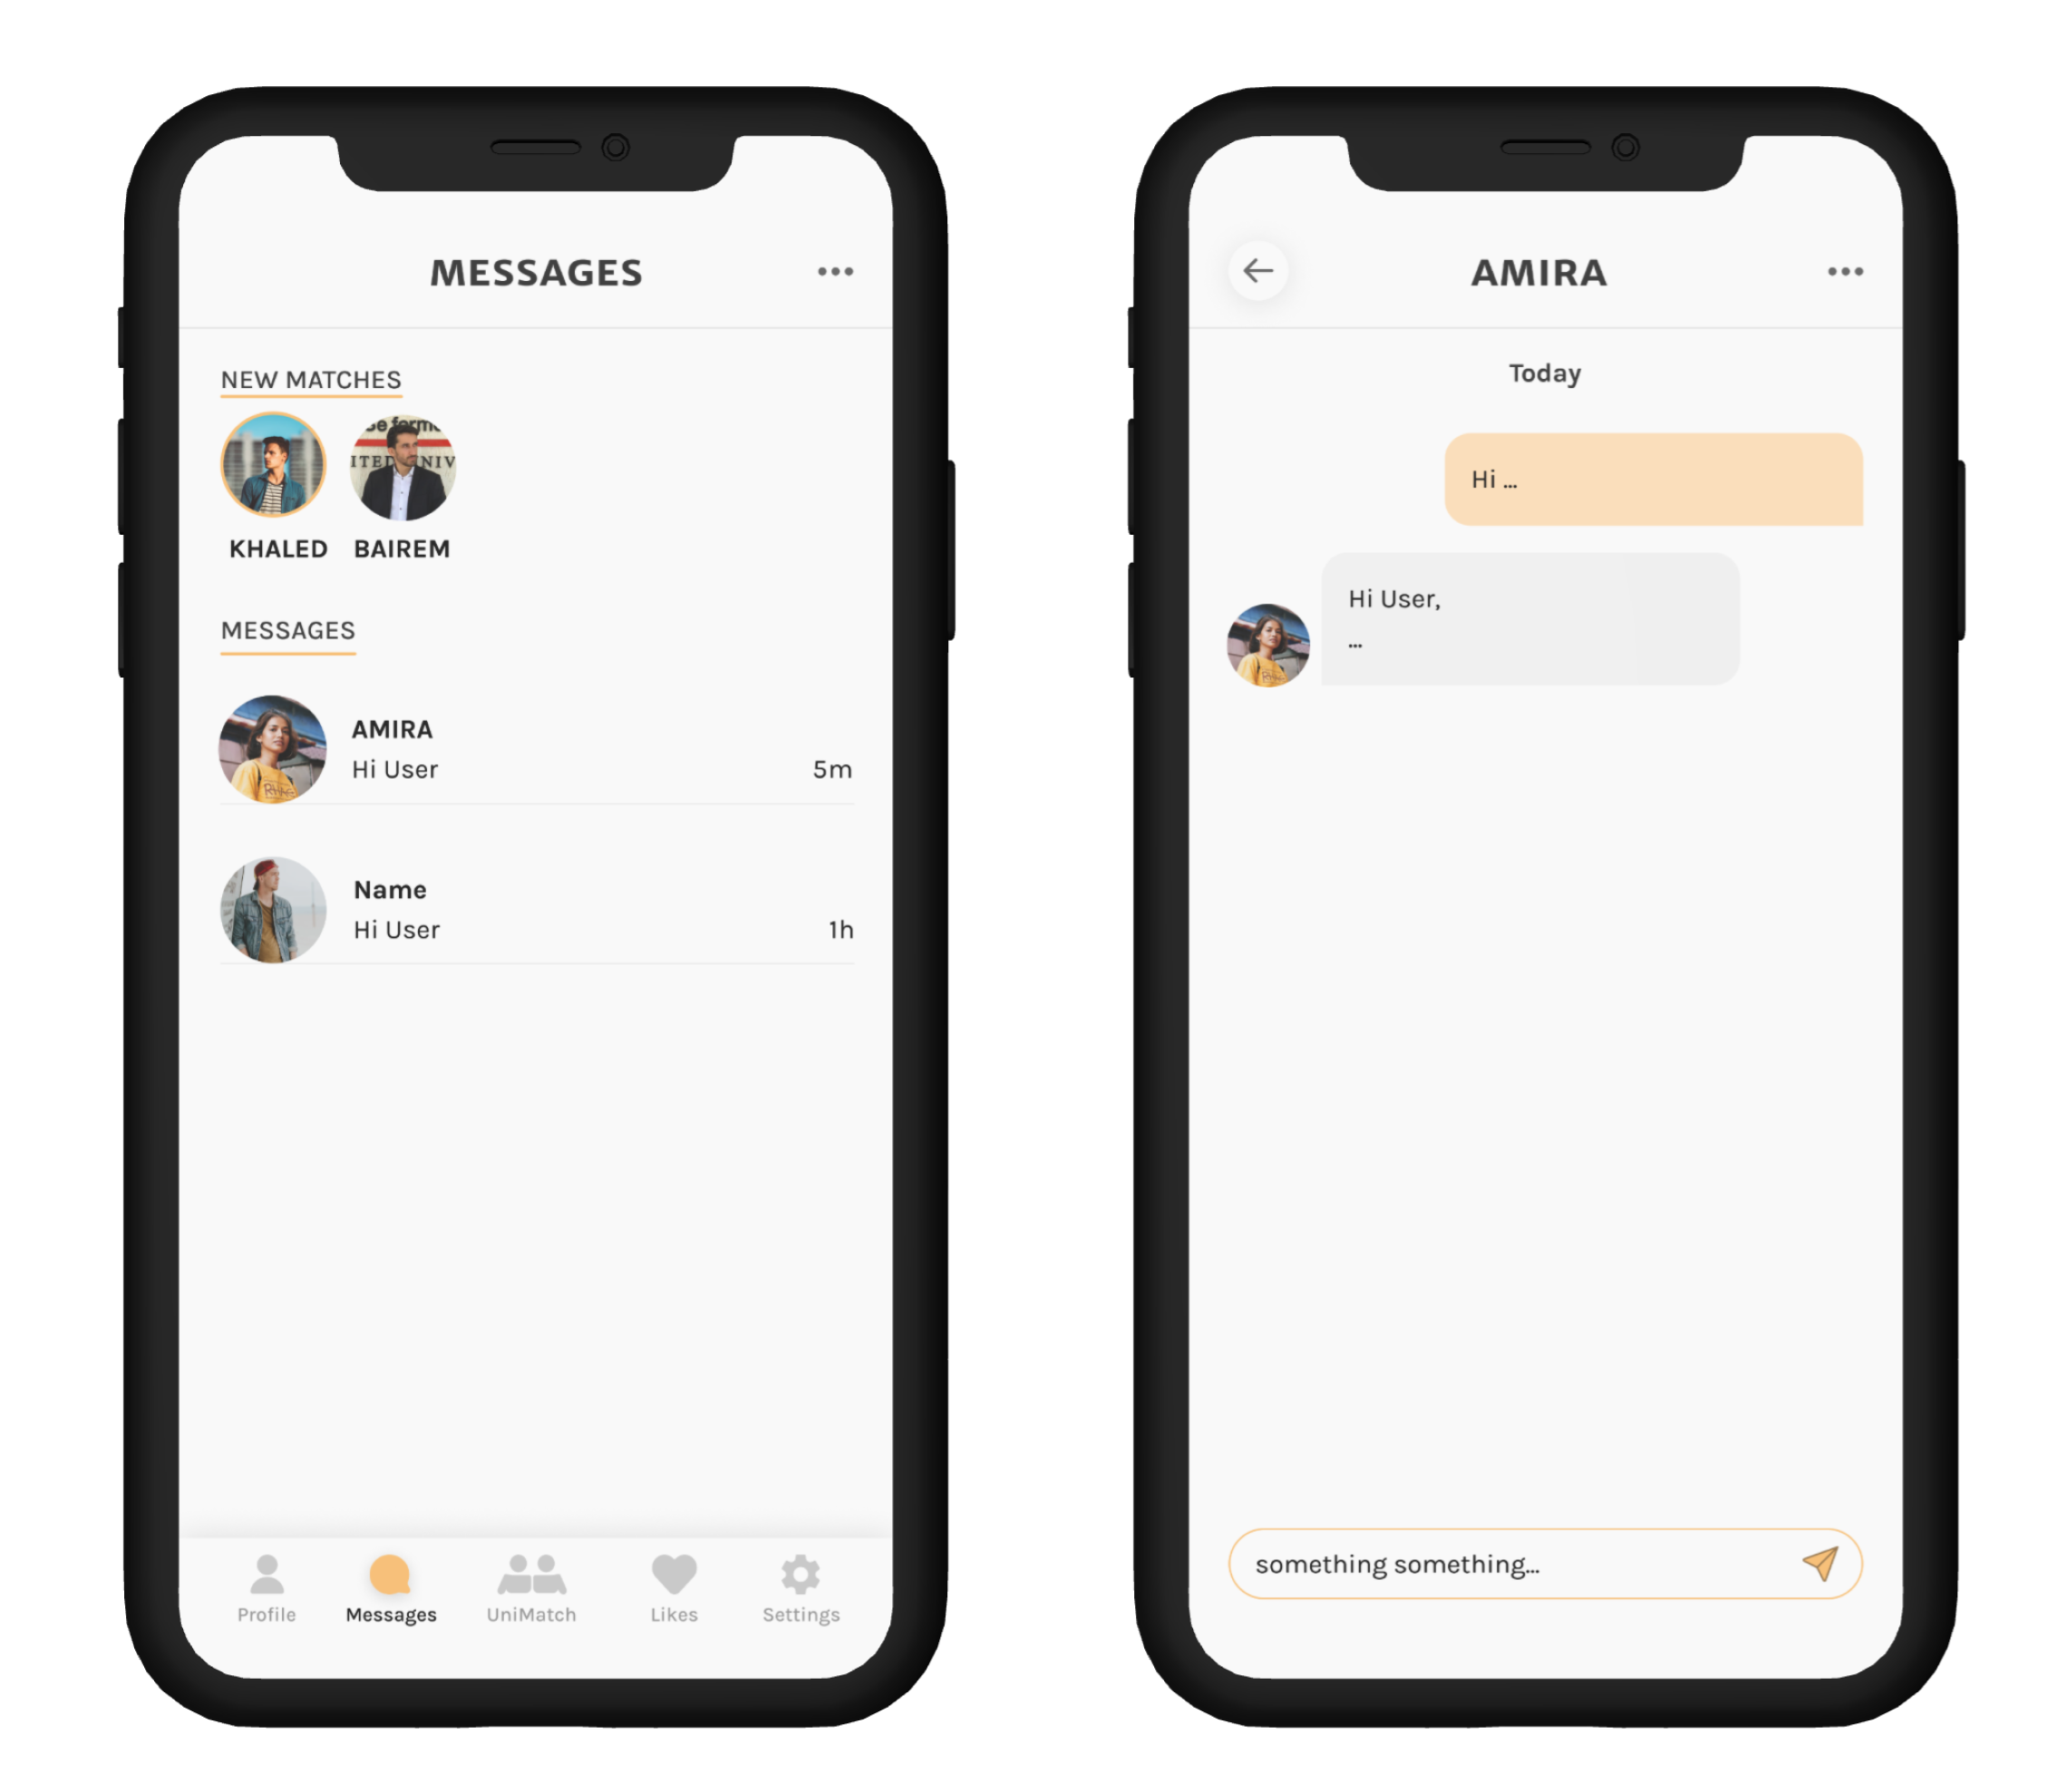
\includegraphics[scale=0.2]{messages ui.png}
            \caption{Messages UI} 
            \label{fig: messages UI}
\end{figure}
\subsection{Likes Management}
After swiping right on a person, they'll notice it in the "Likes" section. In this section, users can guess who likes them by giving them clues about the person who is interested in them. Thanks to these clues, they can find out a little more about the person's personality, which can help them decide whether or not to meet and contact them. \\
In the figure below, we find the "likes" section and on the right- side, we see what happens when we click on one of the "likes" cards to display more details about the person who sent that interest.
\begin{figure}[H] 
            \centering
            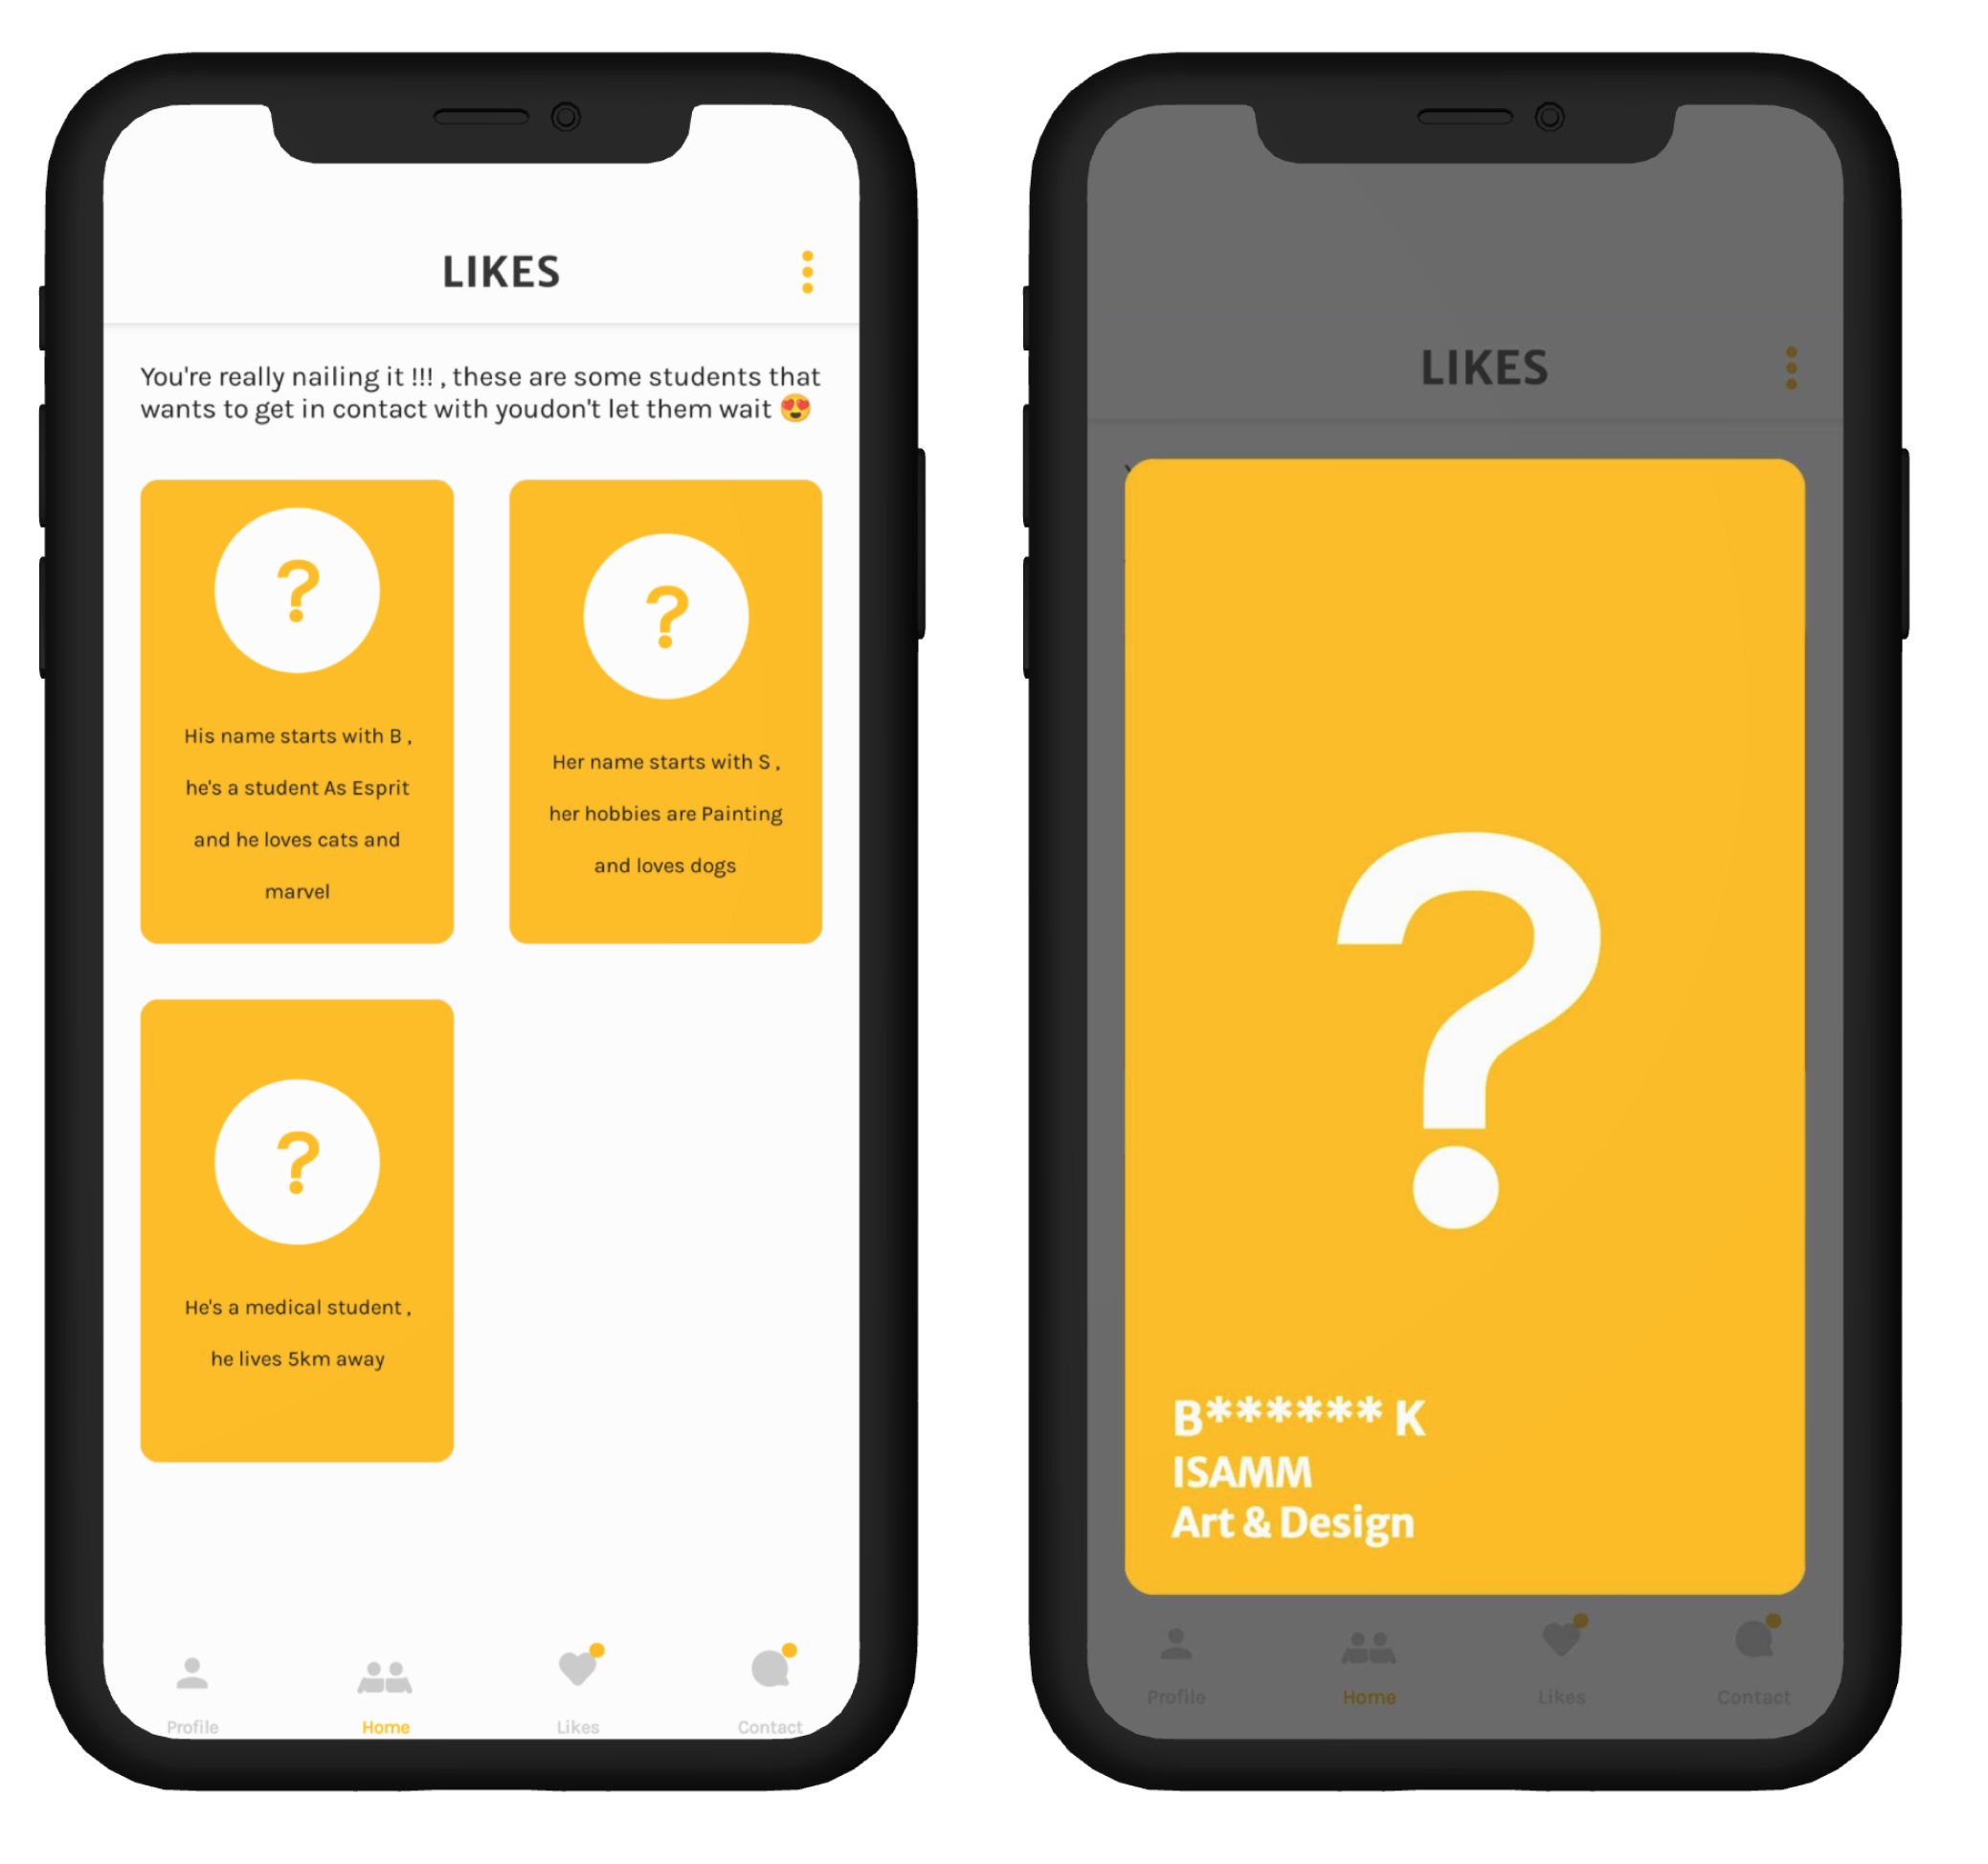
\includegraphics[scale=0.2]{like ui.png}
            \caption{likes management UI} 
            \label{fig: likes management UI}
\end{figure}

\subsection{Filtering Management}
Last but not least, users can choose who they would like to see and have the capability of interacting with them due to a filter option. Users also have a possibility to regulate their potential network with a number of parameters: gender, field of study, university, interests, etc.\\
The following figure is the filtering interface:
\begin{figure}[H] 
            \centering
            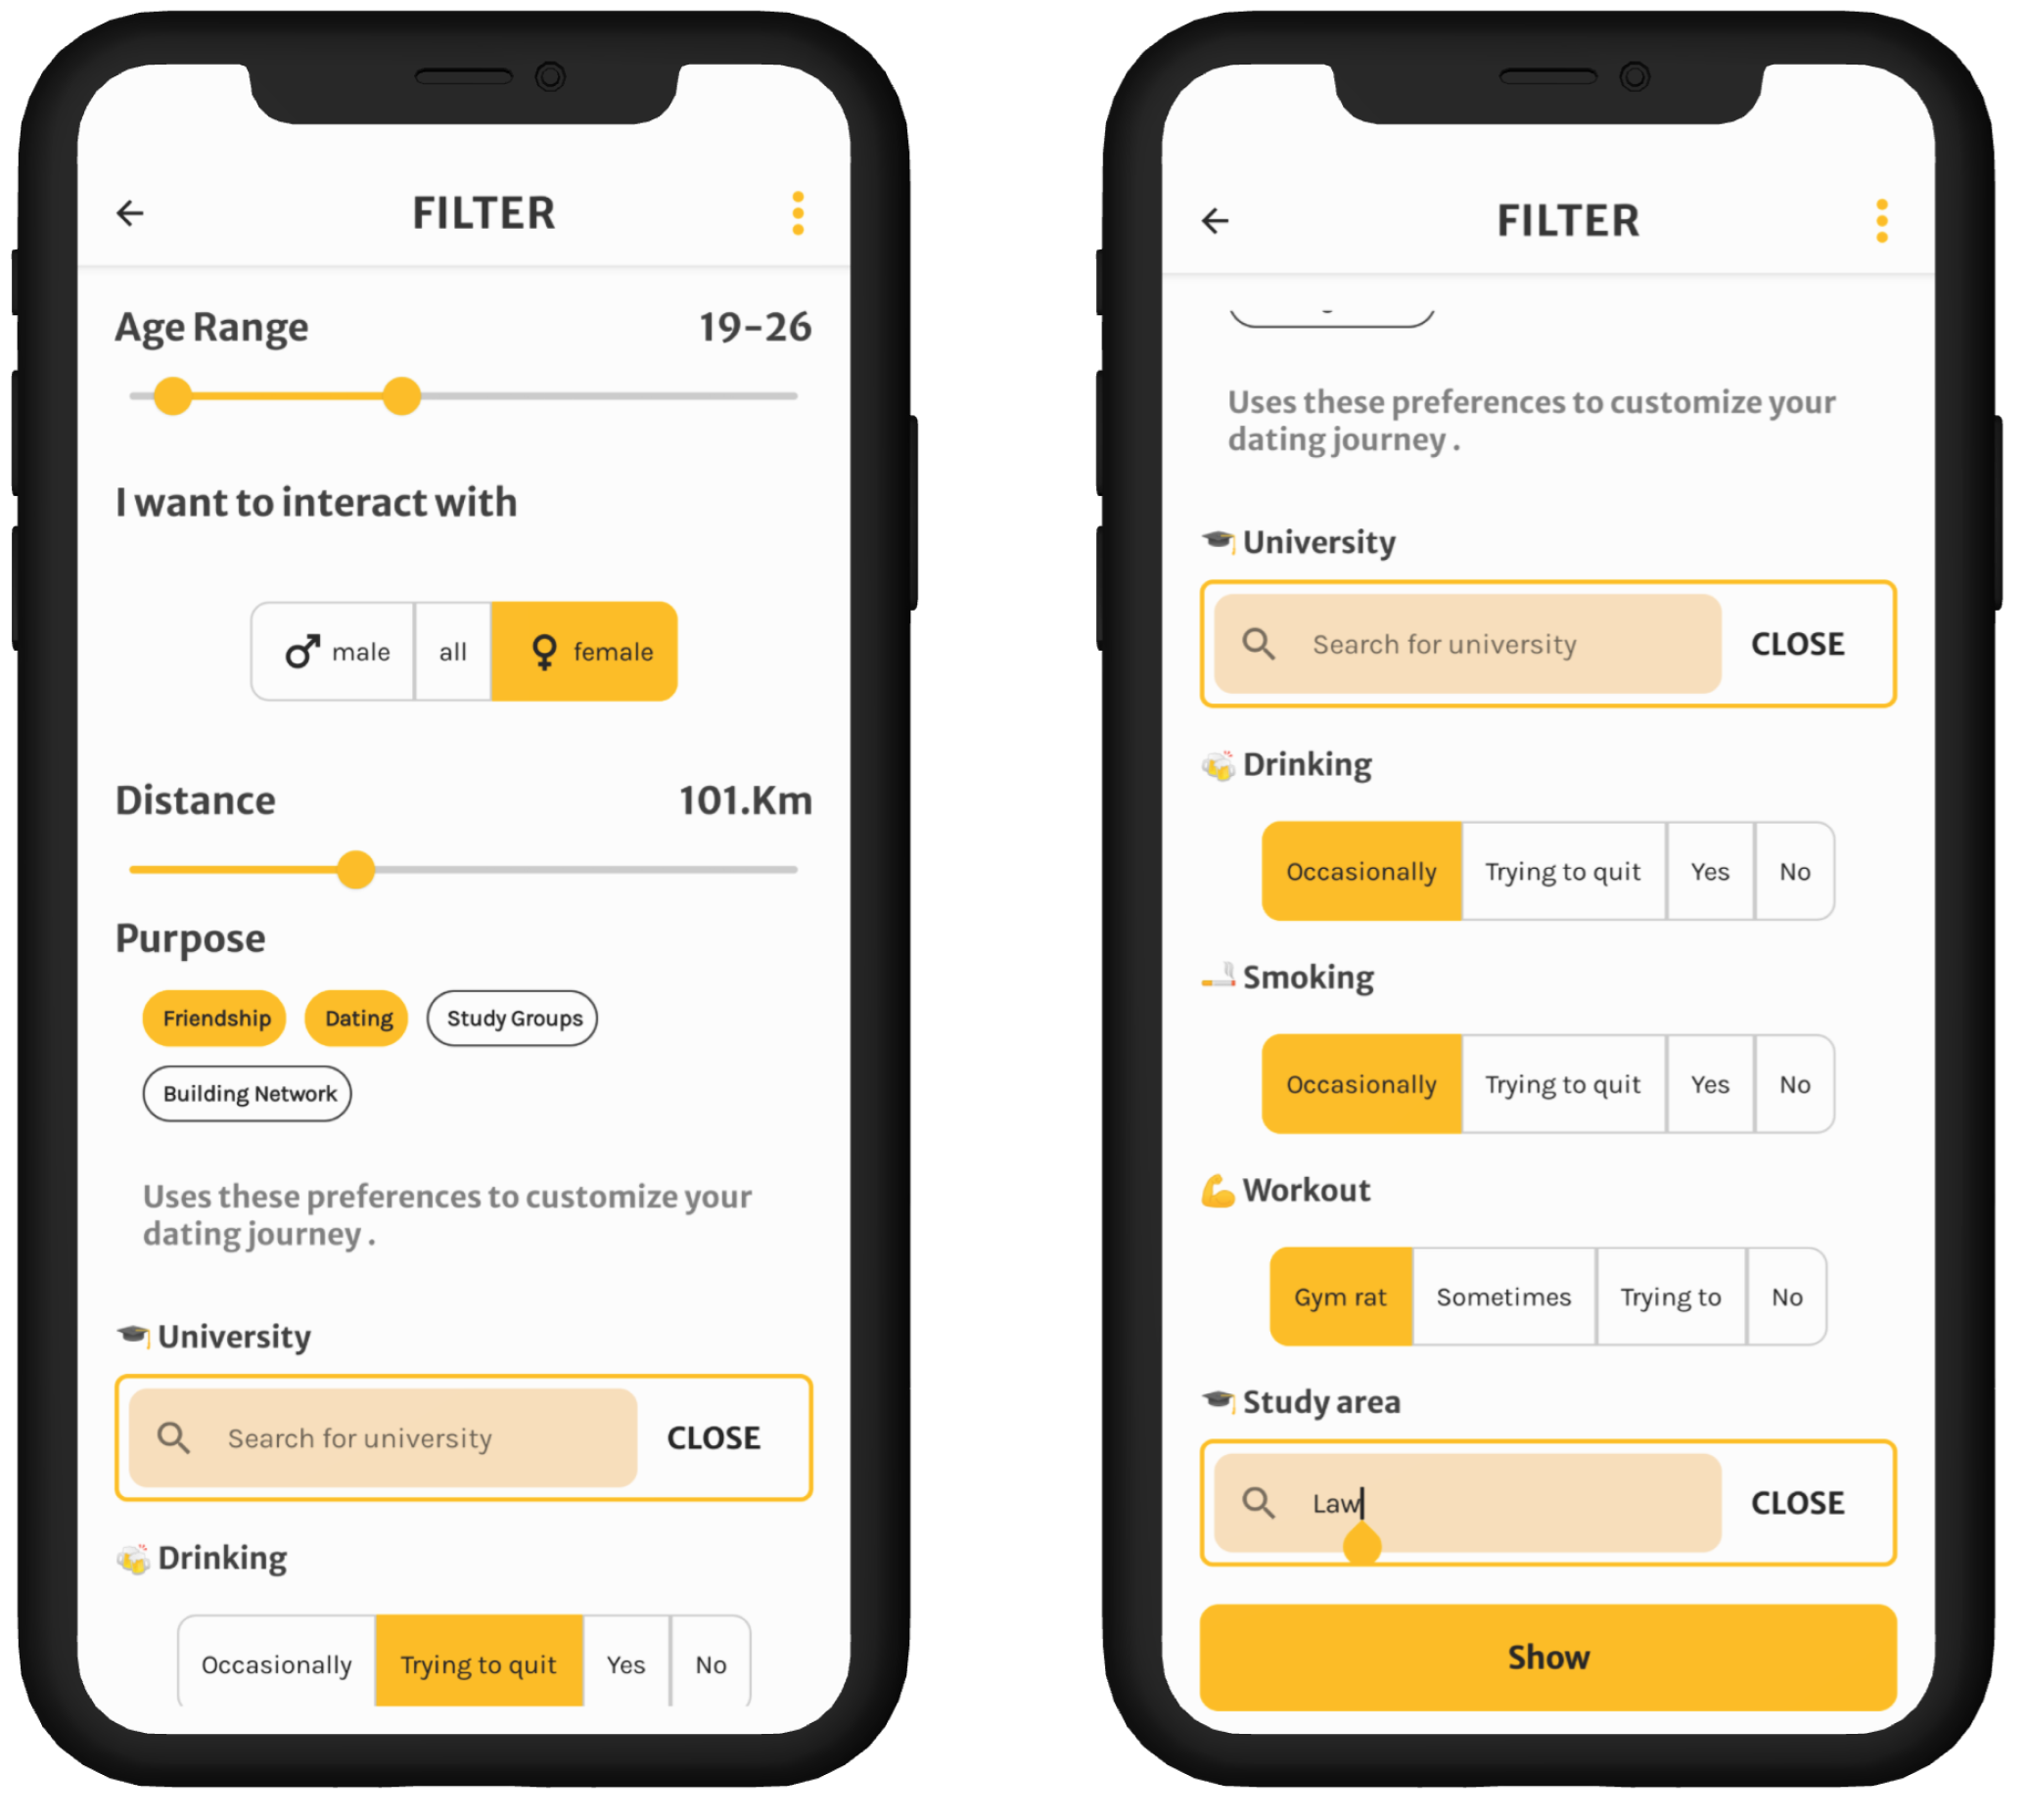
\includegraphics[scale=0.2]{filter ui.png}
            \caption{Feed Filter UI} 
            \label{fig: Feed Filter UI}
\end{figure}

\section*{Conclusion}
\addcontentsline{toc}{section}{Conclusion}
Sticking to the tradition of the chosen methodology, the first sprint introduced a design of the features that are complete for managing users and their authentication. The fact that it is possible to test and specifically these features in the subsequent sprints is the point that brings the team closer to the goal and the great immersive experience. 

